\section{Pilotexperiment}
 \begin{frame}
 	\frametitle{Inhalt}
 	\tableofcontents[%
 		currentsection, % causes all sections but the current to be shown in a semi-transparent way.
% % 		currentsubsection, % causes all subsections but the current subsection in the current section to ...
% % 		hideallsubsections, % causes all subsections to be hidden.
% 		hideothersubsections, % causes the subsections of sections other than the current one to be hidden.
% % 		part=, % part number causes the table of contents of part part number to be shown
% 		pausesections, % causes a \pause command to be issued before each section. This is useful if you
% 		pausesubsections, %  causes a \pause command to be issued before each subsection.
% % 		sections={ overlay specification },
 	]
 \end{frame}
\begin{frame}{Pilotexperiment}
	\begin{itemize}[<+->]
	\item Ziel: überprüfen, ob sich der Biorhythmus eines Probanden mit der App erfassen lässt
	\item Probanden sollten Testreihe über mehrere Tage durchführen
	\item anschließend ähnliche Tests am Rechner um Vergleichswerte zu erhalten
	\item App-Test von 16.11.2011 bis 26.11.2011 Intervall von 150 Minuten
	\item Rechner-Tests von 10.12.2011 bis 12.12.2011 
	\item für Number Pairs keine PC-Implementierung verfügbar
	\item auf PC nur Dual-n-Back verfügbar
	\item PC-Variante erhebt Daten nicht so genau, wie Smartphone-Umsetzung
	\end{itemize}
\end{frame}
\begin{frame}{Ergebnisse}
	\begin{figure}[hbtp]
	\centering
	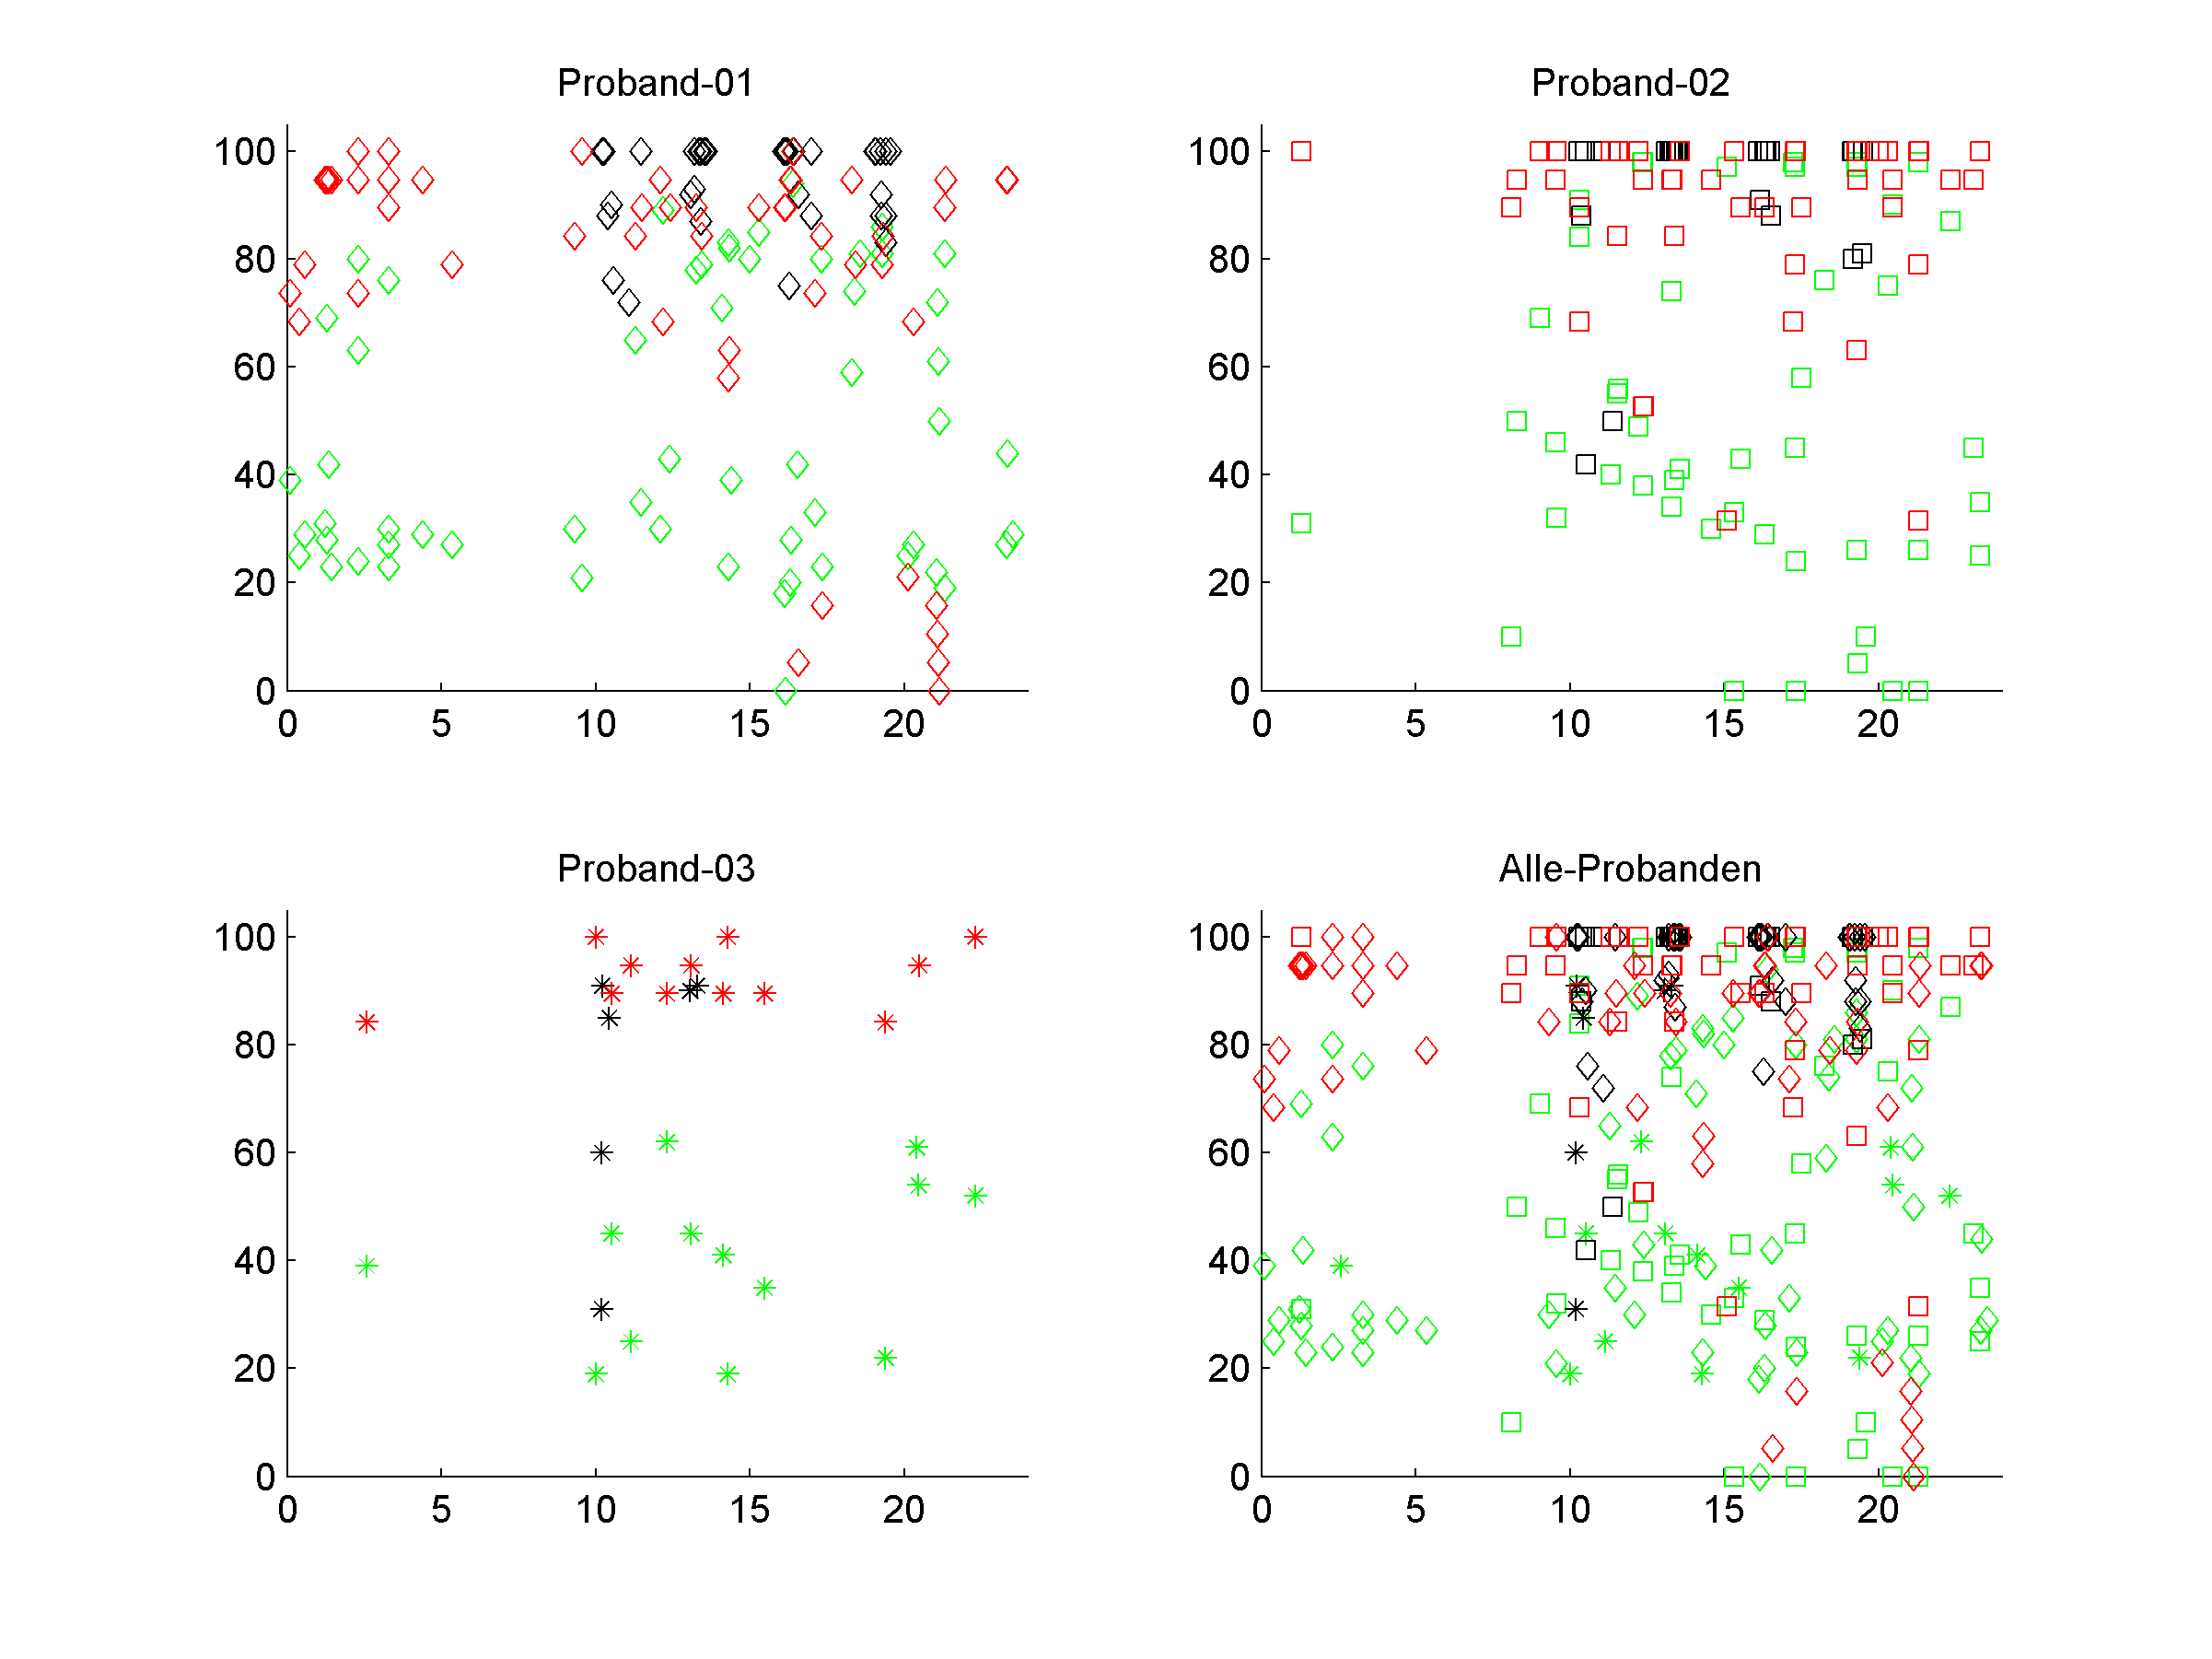
\includegraphics[width=0.8\linewidth]{pictures/NBack_Uebersicht}
	
	\label{fig:results_first_experiment}
	\end{figure}
\end{frame}

\begin{frame}
\begin{figure}[htbp]
\centering
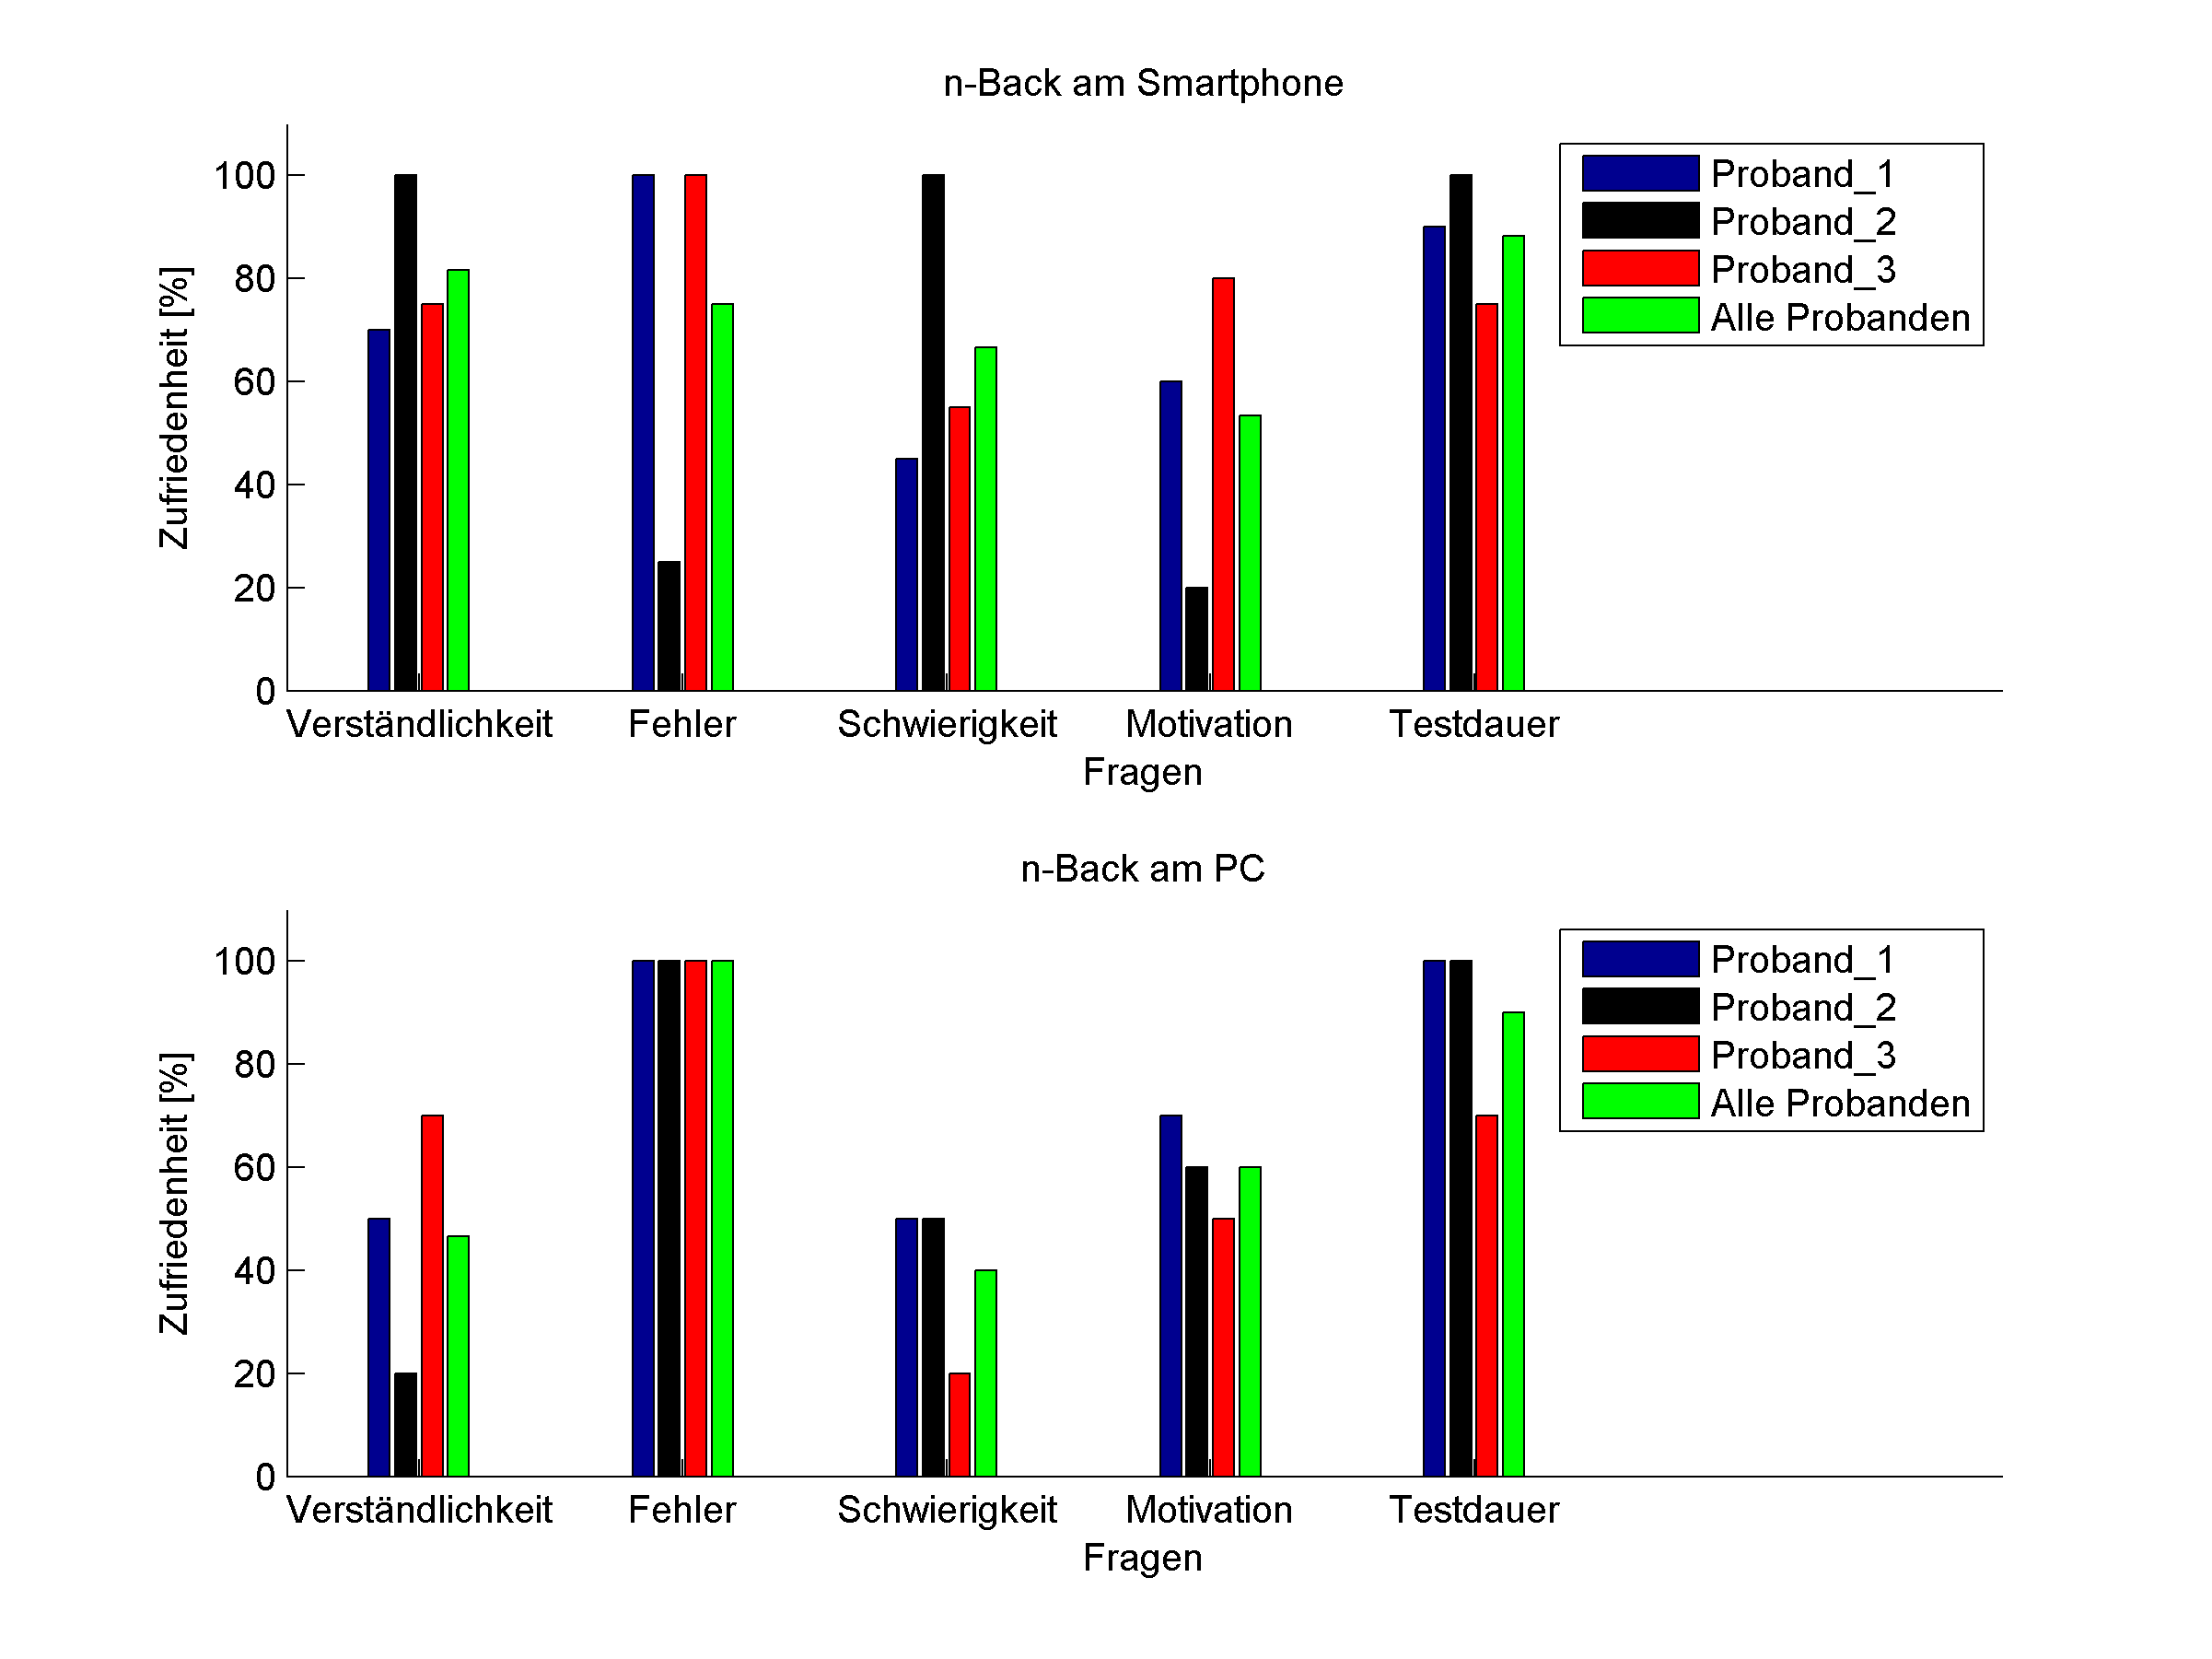
\includegraphics[width=0.9\linewidth]{pictures/NBACK_Fragebogen}
\label{fig:question-n-back}
\end{figure}

\end{frame}
\begin{frame}
\begin{figure}
\centering
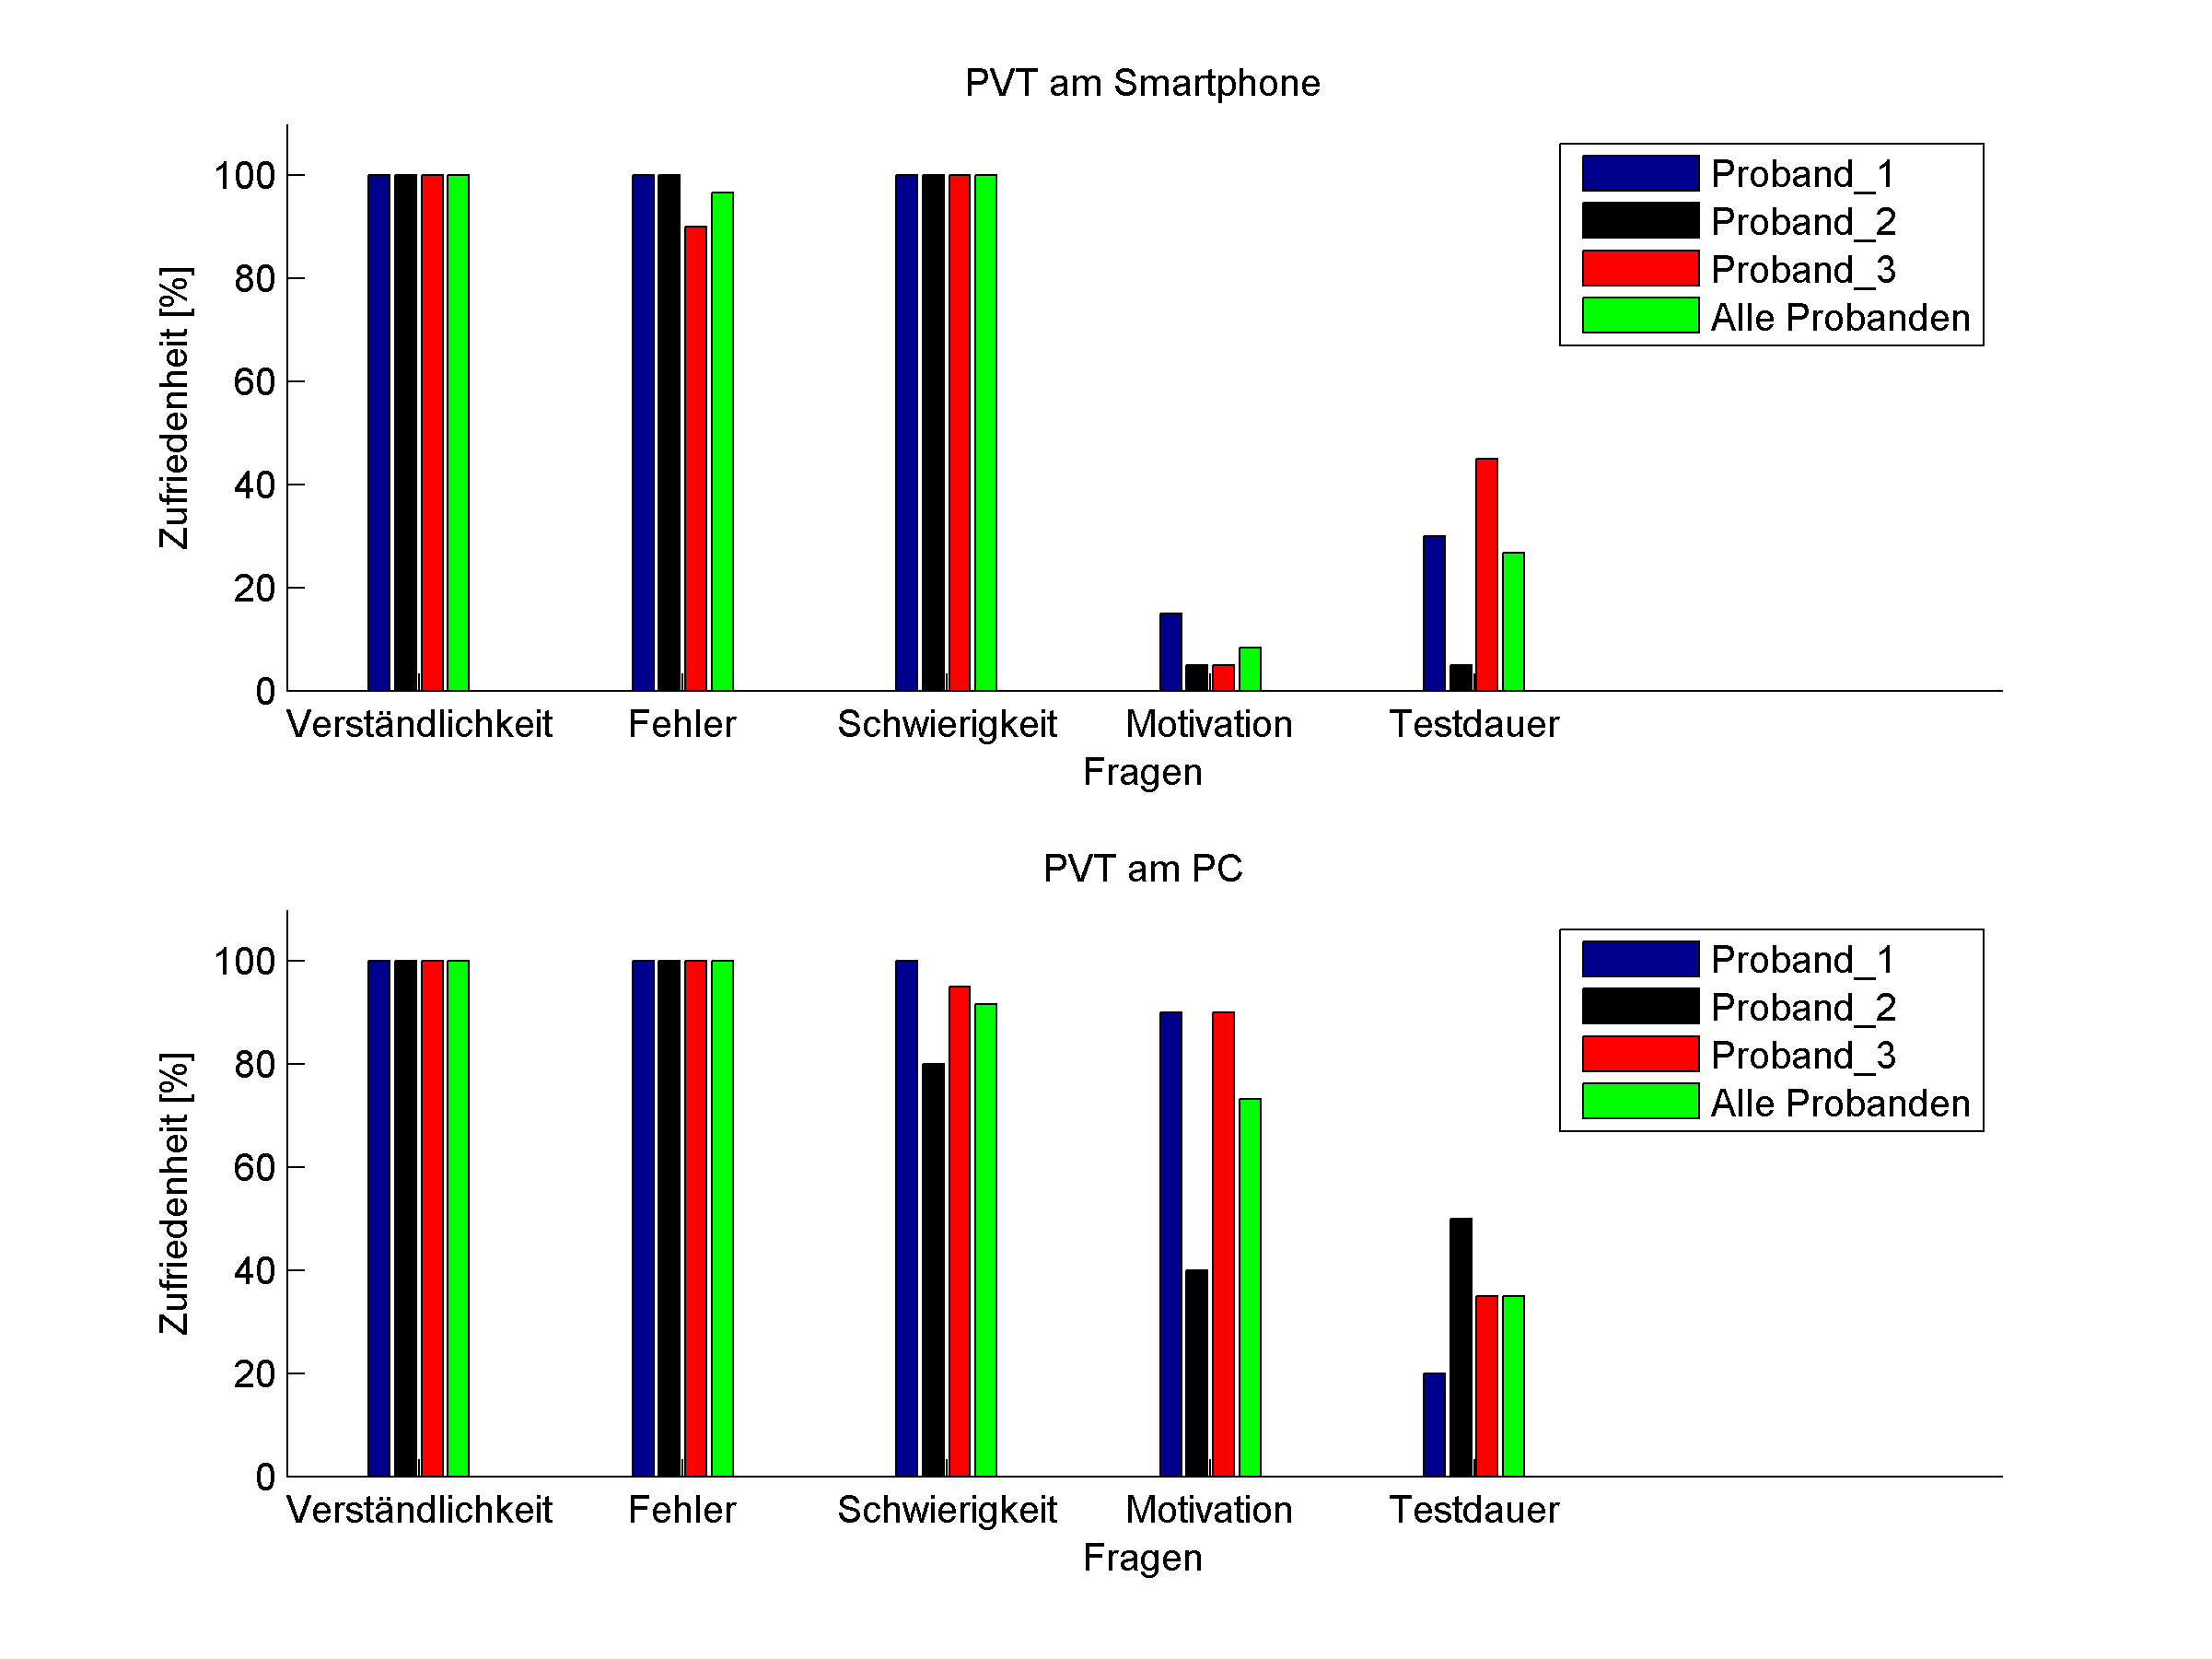
\includegraphics[width=0.9\linewidth]{pictures/PVT_Fragebogen}
\label{fig:question-pvt}
\end{figure}
\end{frame}
\begin{frame}{Zweite Studie}
	\begin{itemize}[<+->]
	\item nicht erhoffte Ergebnisse
	\item daher zweite Studie
	\item Ziel: Vergleichbare Resultate
	\item zwei Probanden ähnliche Tests über 10 Stunden
	\item eine Testreihe pro Stunde
	\item erst PC-Test danach Smartphone-Test
	\end{itemize}
\end{frame}

\begin{frame}
\begin{figure}[hbtp]
 \centering
 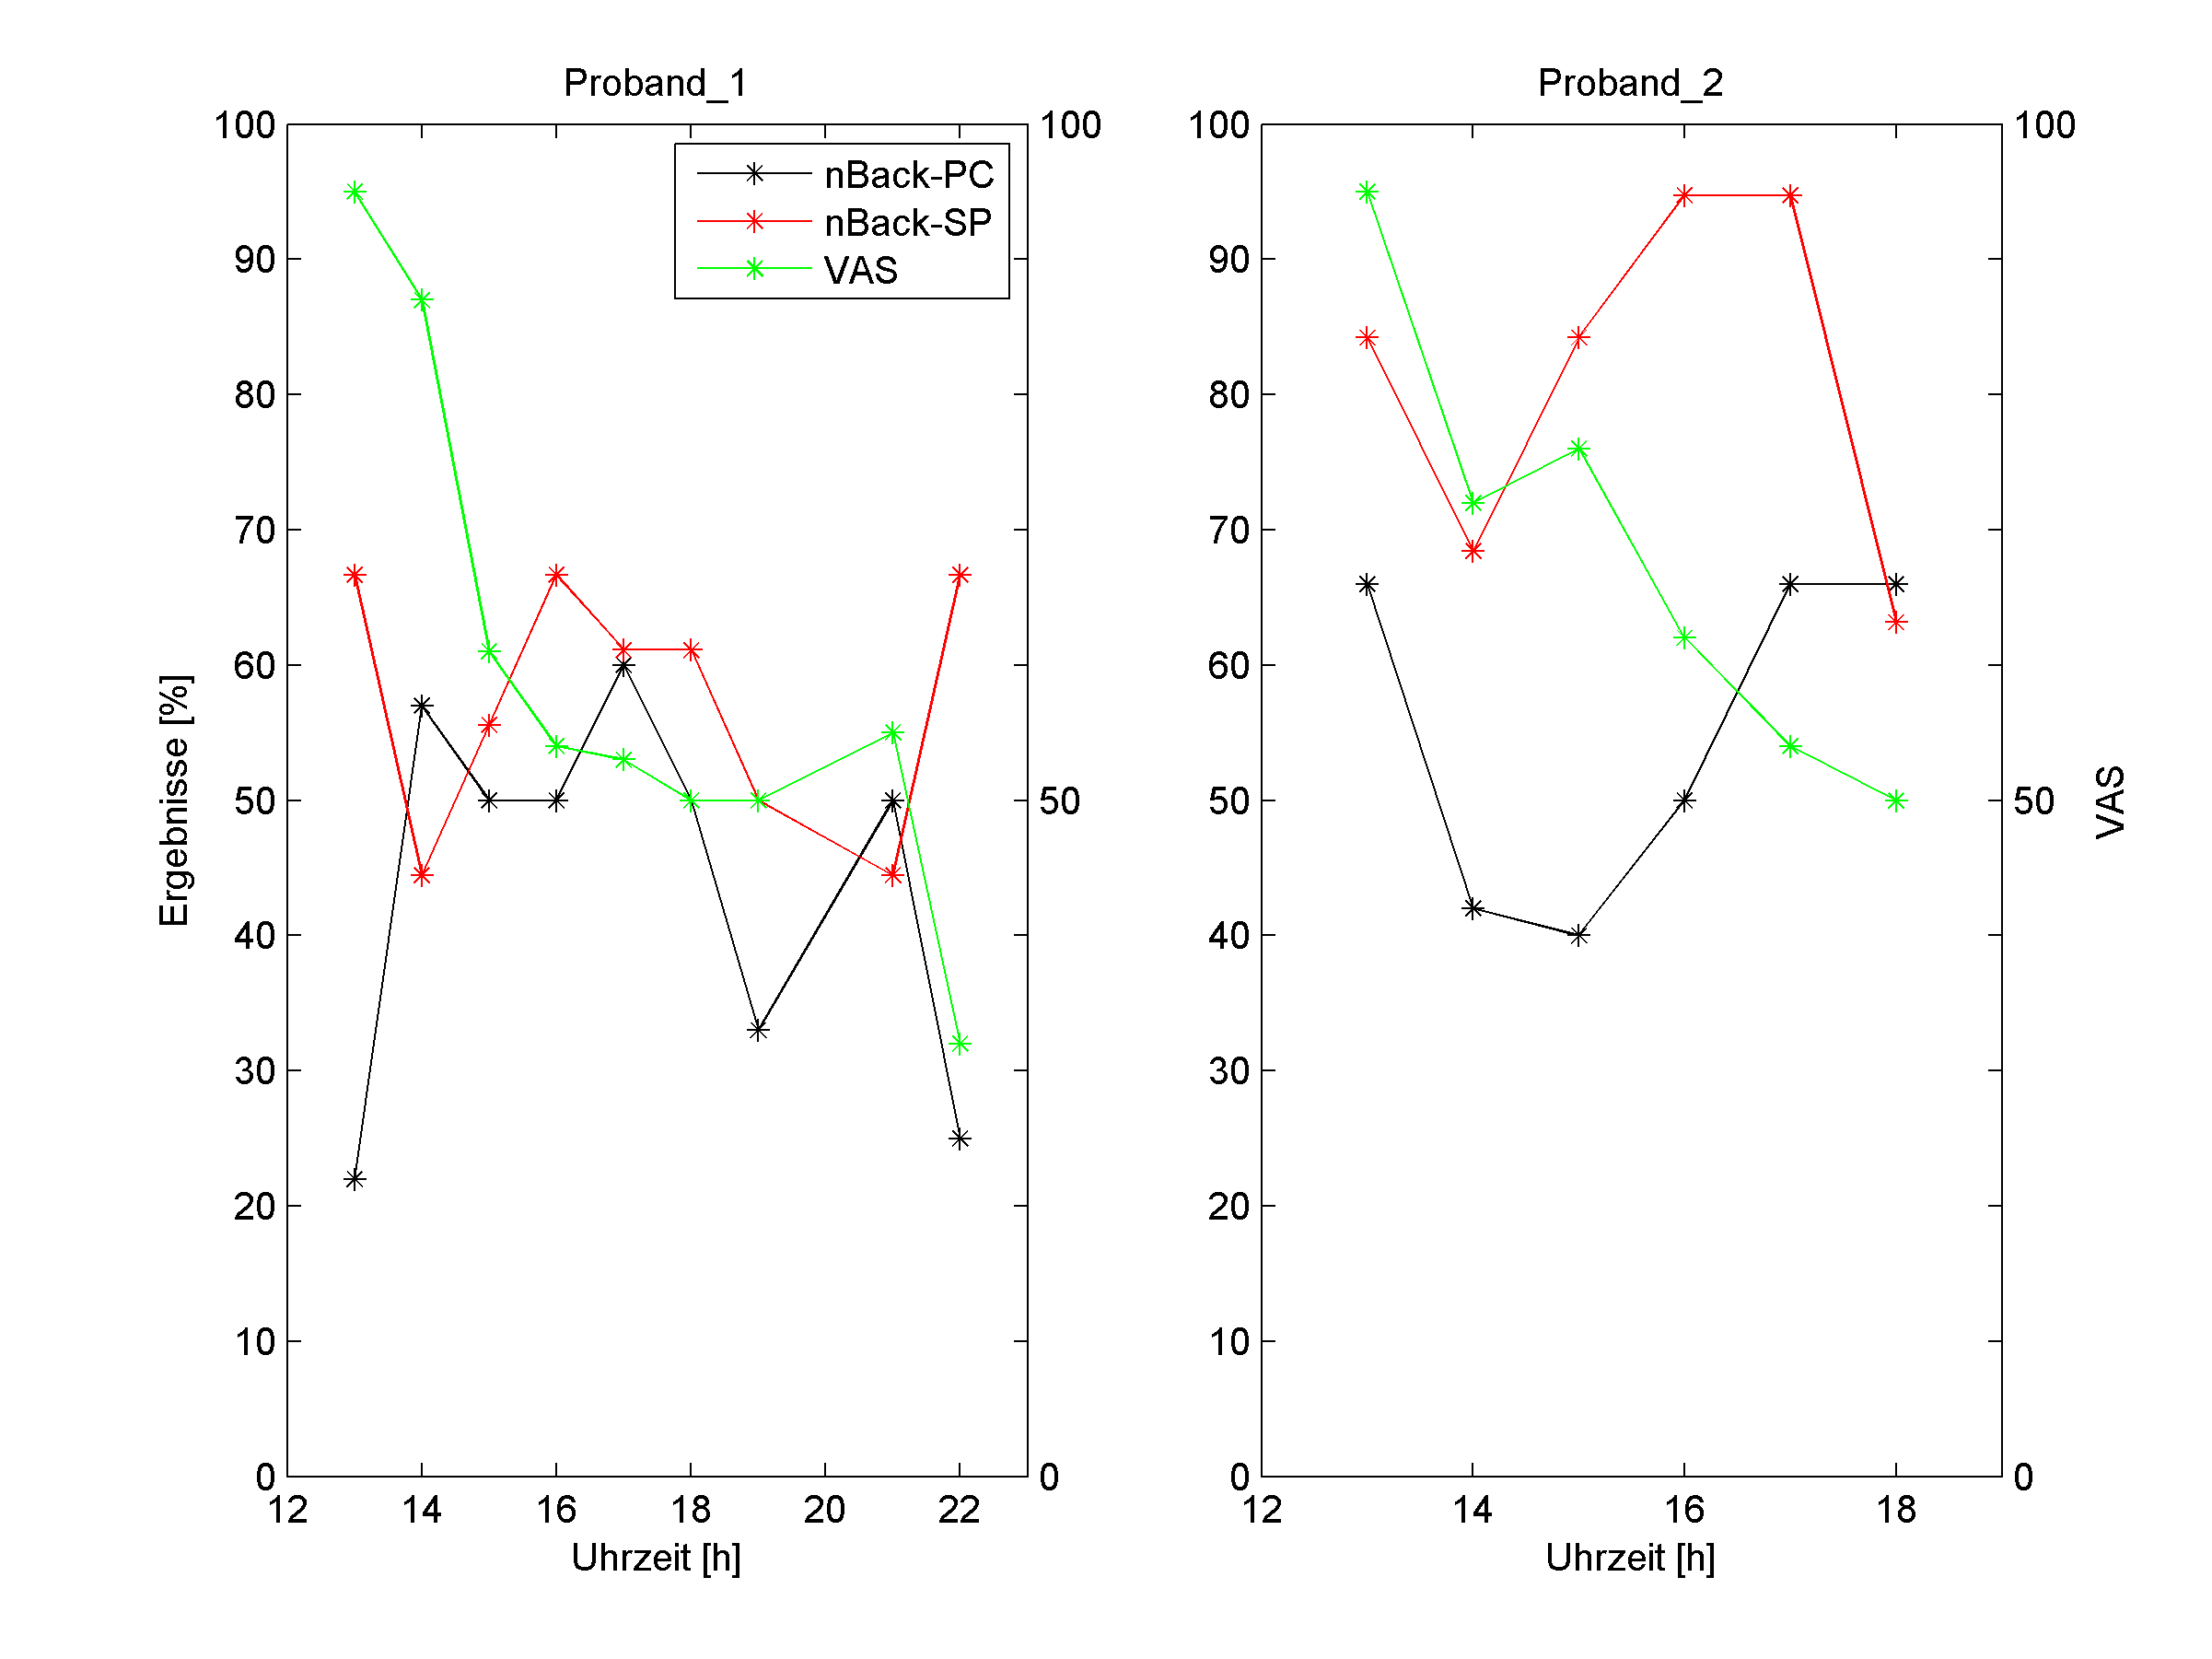
\includegraphics[width=0.9\linewidth]{pictures/n-back_results}

 \label{fig:studie2-n-back}
\end{figure}

\end{frame}
\begin{frame}
\begin{figure}
 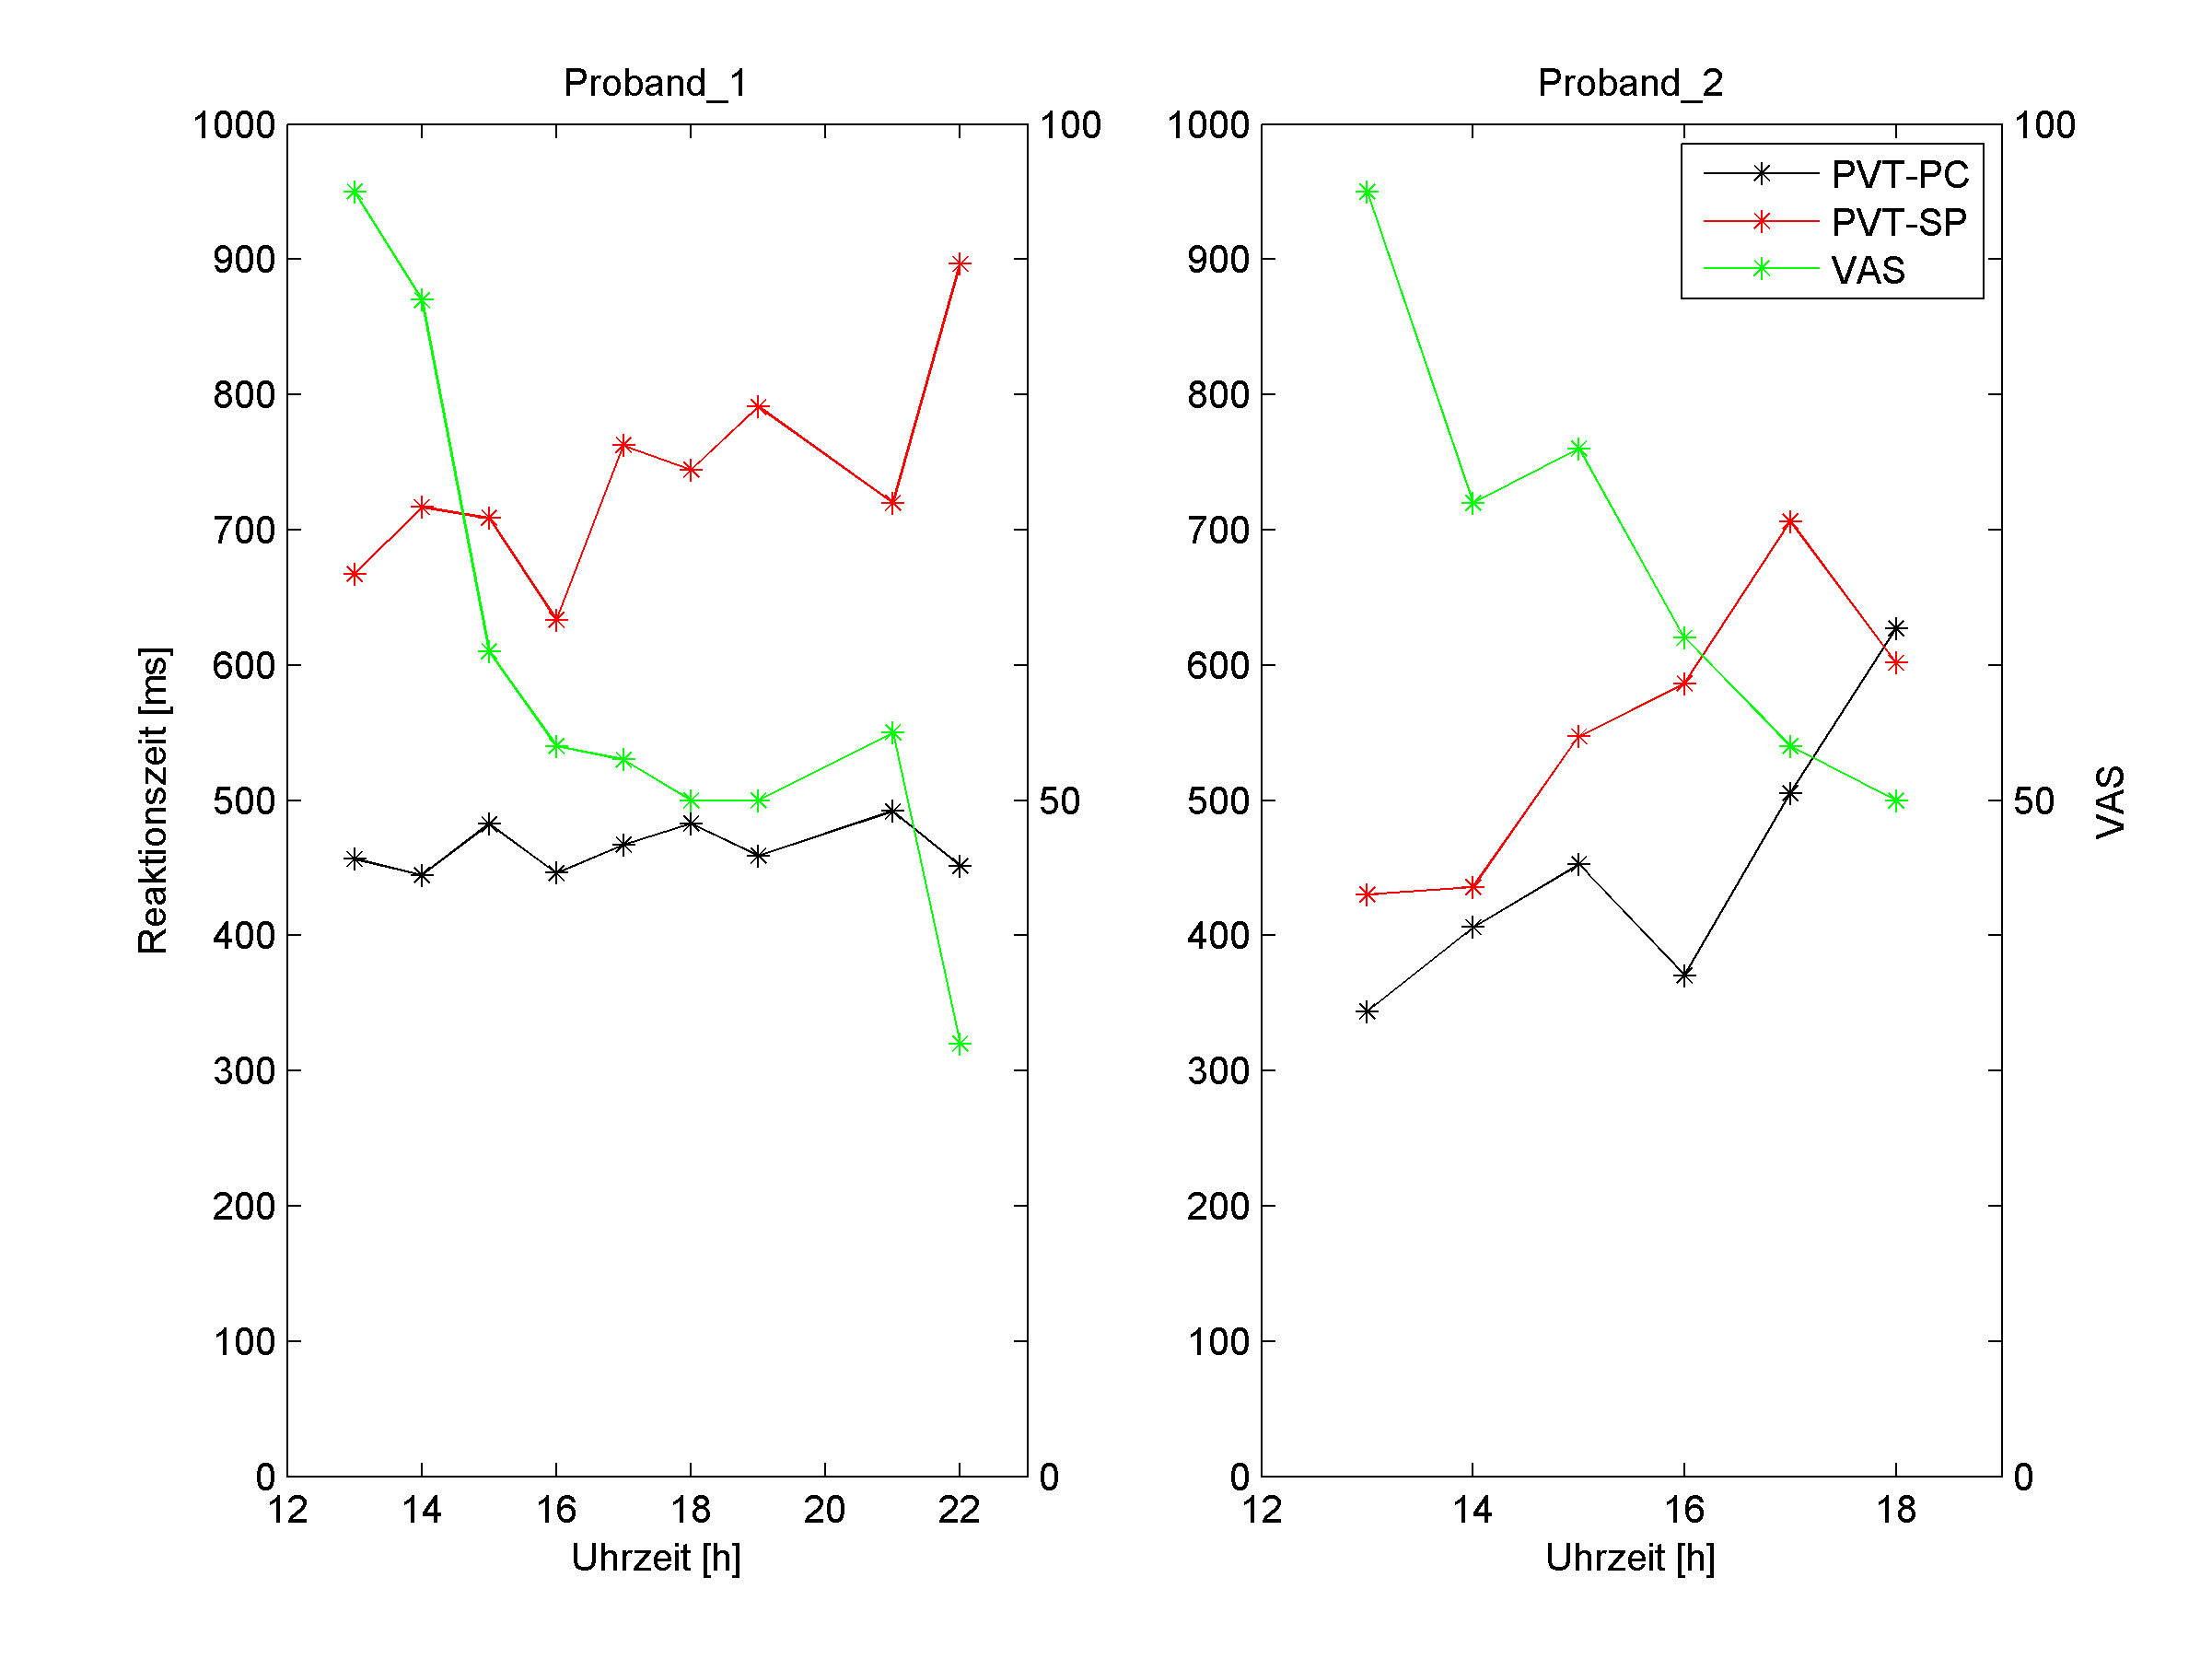
\includegraphics[width=0.9\linewidth]{pictures/pvt_results}

 \label{fig:studie2-pvt}
 \end{figure}

\end{frame}
